
%%%%%%%%%%%%%%%%%%%%%%%%%%%%%%%%%%%%%%%%%%%%%%%%%%%%%%%%%%%%
%
% Section: Solving Equations Graphically
%
%%%%%%%%%%%%%%%%%%%%%%%%%%%%%%%%%%%%%%%%%%%%%%%%%%%%%%%%%%%%

\section{Solving Equations Graphically}
\label{SolvingEquationsGraphically}

Graphs are a powerful tool which we will exploit throughout this book. A particularly powerful use for graphs is as a tool to solve equations, particularly in cases where traditional algebra methods would be tedious or ineffective. In this chapter we will introduce this method and discuss when it is - and when it is not - a useful alternative.

%%%%%%%%%%%%%%%%%%%%%%%%%%%%%%%%%%%%%%%%%%%%%%%%%%%%%%%%%%%%
%
% SubSection: Solving Equations Graphically:Graphical Solution
%
%%%%%%%%%%%%%%%%%%%%%%%%%%%%%%%%%%%%%%%%%%%%%%%%%%%%%%%%%%%%

\subsection{Graphical Solution}

We’ll begin this chapter by showing how we could use a graph to solve a fairly simple equation.
Consider, for example, the equation:

\begin{equation*}
	2x-1=7
\end{equation*}

Now, it is not hard to solve this equation with traditional algebra. Add one to both sides, divide by two, and you can quickly conclude that the solution is $x=4$. Fair enough. But we also could have seen this in another way.\\

The algebraic expression on the left side of that equation can be used to define a function, $f(x)=2x-1$. Using the calculator, we can readily obtain a graph of this function (shown below in the standard window):

\begin{figure}[H]
	\centering
	%should be scaled down
	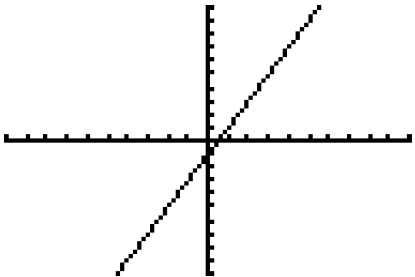
\includegraphics[scale=1.0]{Sections/SolvingEquationsGraphically/Figure01.png}
	\caption{Graph of $f(x)=2x-1$ in the standard window}
\end{figure}

Now, remember that a graph for a function consists of all of its input-output pairs. For example, $(5,9)$ lies on this graph, because when you input $x=5$ into the function $f(x)=2x-1$ the resulting output is $f(5)=9$.\\

Now, solving the equation $2x-1=7$ amounts to asking \quotes{what $x$ value do we need to input into $f(x)=2x-1$ to get $7$ as the resulting output?} We can find this by looking for the point on the graph where the output value is $7$; that is, where $f(x)=7$.\\

We could try to do this by tracing along the graph to get to the point we are seeking, but we can find it more efficiently in another way. If we consider the right side of the equation as also defining a function $g(x)=7$ and graph that function, the result is just a flat horizontal line whose output value stays at $7$ no matter where we go on the input axis (shown below in the standard window):

\begin{figure}[H]
	\centering
	%should be scaled down
	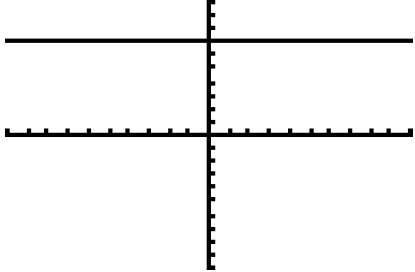
\includegraphics[scale=1.0]{Sections/SolvingEquationsGraphically/Figure02.png}
	\caption{Graph of $g(x)=7$ in the standard window}
\end{figure}

Now, we can graph the right-side function and left-side function together. The \quotes{Y=} screen allows us to enter more than one function at once, so if we do this:

\begin{figure}[H]
	\centering
	%should be scaled down
	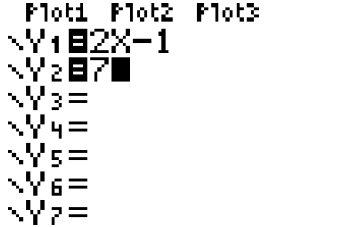
\includegraphics[scale=1.0]{Sections/SolvingEquationsGraphically/Figure03.png}
	\caption{Entering two function in the calculator}
\end{figure}

And then we get both graphed together in the same window:

\begin{figure}[H]
	\centering
	%should be scaled down
	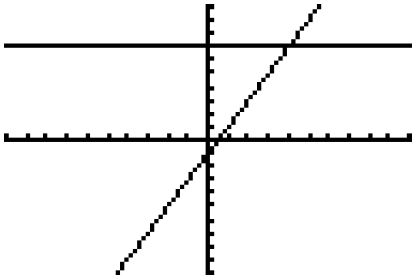
\includegraphics[scale=1.0]{Sections/SolvingEquationsGraphically/Figure04.png}
	\caption{Graph of $f(x)=2x-1$ and $g(x)=7$ in the standard window}
\end{figure}

Now, how does this help? Well, we are looking for the place where the output of $f(x)=2x-1$ is $7$ -- or, in other words, where the graph of $f(x)=2x-1$ is at a height of $7$. But the output of $g(x)=7$ is always $7$, or, in other words, the graph of $g(x)=7$ is always at a height of $7$. So, the point on the graph of $f(x)=2x-1$ that we are looking for is the point where the two graphs intersect!\\

The calculator has programs built in to find the intersection between two graphs. We’ll walk through that right now, step-by-step.\\

\index{Calculator:Intersection}In the top row of your calculator, you will see a key labeled \quotes{TRACE} which is marked above as \quotes{CALC}. Hit \quotes{2nd} and then this key to reach the \quotes{CALC} menu. You should see this:

\begin{figure}[H]
	\centering
	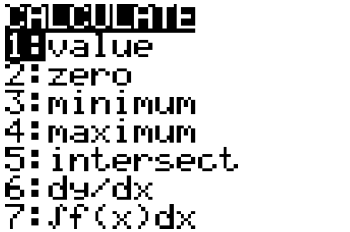
\includegraphics[scale=1.0]{Sections/SolvingEquationsGraphically/Figure05.png}
	\caption{The \quotes{CALC} menu}
\end{figure}

Now, select \quotes{5: Intersect} and the graphs will appear:

\begin{figure}[H]
	\centering
	%should be scaled down
	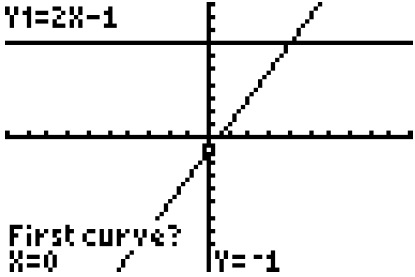
\includegraphics[scale=1.0]{Sections/SolvingEquationsGraphically/Figure06.png}
	\caption{The first step toward finding the intersection}
\end{figure}

Now we are ready to work through the calculator program to find the intersection. Because the calculator can store more than two graphs, the program first asks you to confirm which two graphs you want to intersect. (Unfortunately, you still have to do this even if you’ve only entered two!) The \quotes{First curve?} question at the bottom of the screen is asking you to confirm that one of the two graphs you want to intersect is indeed the one shown in the upper left-hand corner, \quotes{Y1=2X-1}.
(The word \quotes{curve} is an old-fashioned word for graph; for our purposes you can just read this as meaning the same thing as \quotes{graph}.) Since this is correct, you only need to hit \quotes{Enter} to confirm.  The screen should now show this:

\begin{figure}[H]
	\centering
	%should be scaled down
	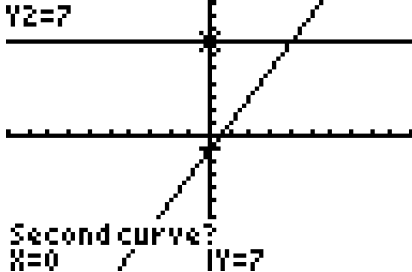
\includegraphics[scale=1.0]{Sections/SolvingEquationsGraphically/Figure07.png}
	\caption{The second step toward finding the intersection}
\end{figure}

Since \quotes{Y2=7} is indeed the other graph, hit \quotes{Enter} again to confirm.

\begin{figure}[H]
	\centering
	%should be scaled down
	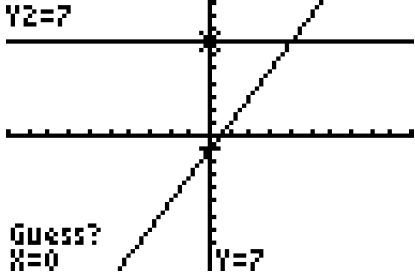
\includegraphics[scale=1.0]{Sections/SolvingEquationsGraphically/Figure08.png}
	\caption{The third step toward finding the intersection}
\end{figure}

The calculator is now asking for a guess. The calculator will find the intersection that is closest to the guess you enter here. Since there is only one intersection, this doesn’t really matter, though when there is more than one intersection (which we will see an example of shortly) this step is important. Here, you can use the arrow keys to move the blob closer to the intersection if you like, but you can also just hit \quotes{Enter} without changing anything and let it go:

\begin{figure}[H]
	\centering
	%should be scaled down
	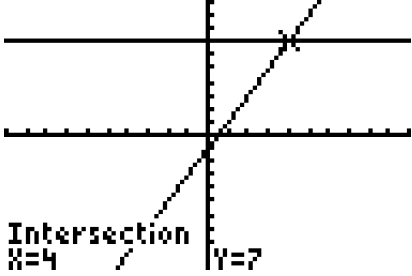
\includegraphics[scale=1.0]{Sections/SolvingEquationsGraphically/Figure09.png}
	\caption{Found the intersection}
\end{figure}

So the intersection occurs at $(4,7)$. Our goal though was to solve the original equation, so this is not quite the answer we were looking for. We set these graphs up so that the input ($x$) value of their intersection would be the solution to the original equation. So, we conclude that the solution is:

\begin{equation*}
	x=4
\end{equation*}

which agrees with the answer we got solving using traditional algebra.\\

Now, the equation in this example we’ve worked through was quite simple, chosen just to illustrate how the method works. Given the choice, you’d almost certainly not choose to use graphical solution for this one, since traditional algebra would have been much less work. The point, though, is that the graphing method works just as well if the algebra to solve the equations would be more demanding. We’ll illustrate this with a few examples.

\exam{\label{SolvingEquationsGraphicallyExample1} Solve $t+2=4(2t+1)-2(3t-1)$}

\indenttext{We begin by making each side of the equation a function, and entering them into the calculator.  Remember that in the calculator the input variable must always be rewritten as \quotes{X}. So we enter:
	\begin{figure}[H]
		\centering
		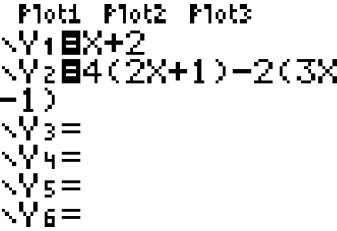
\includegraphics[scale=1.0]{Sections/SolvingEquationsGraphically/Figure10.png}
		\caption{Entering both sides of the equation}
	\end{figure}
	
	Running through the steps:
	
	\begin{enumerate}
		\item Select \quotes{2nd} \quotes{TRACE} (i.e. \quotes{CALC}) --> \quotes{5:Intersect}
		\item Hit \quotes{Enter} to confirm we want to use Y1=X+2
		\item Hit \quotes{Enter} to confirm we want to use Y2=4(2X+1) – 2(3X – 1)
		\item Hit \quotes{Enter} to agree to the suggested guess
	\end{enumerate}
	
	We end up with:
	
	\begin{figure}[H]
		\centering
		%should be scaled down
		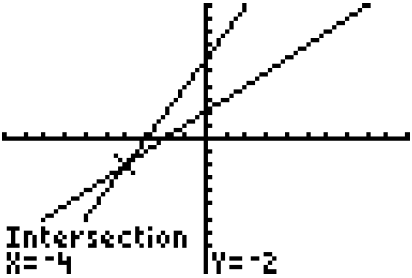
\includegraphics[scale=1.0]{Sections/SolvingEquationsGraphically/Figure11.png}
		\caption{The intersection on the calculator}
	\end{figure}
	
	From this we use the X-value of the intersection to conclude that the solution to the equation is $t=-4$\\
	
	We can check this is by substituting it back into the original equation. (It’s not a bad idea to do this, since even though the calculator will never make an error in finding the intersection, it is always possible that you might make a typographical error entering the formulas.)
}

\exam{\label{SolvingEquationsGraphicallyExample2} Solve $x^2-10=2x$.  Round to two decimal places if necessary.  This equation has two solutions.}

\indenttext{
	Now, this is actually a problem that we cannot (yet) solve using traditional algebra, because if we try to put the $x$ terms together we are unable to do so, because we cannot put the $x^2$ and $2x$ together – they are unlike terms.  Graphical solution still works just fine though.\\

	Starting with:

	\begin{figure}[H]
		\centering
		%should be scaled down
		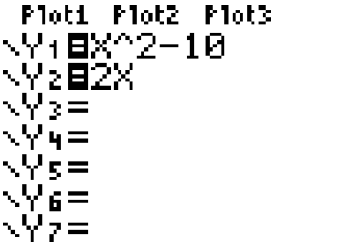
\includegraphics[scale=1.0]{Sections/SolvingEquationsGraphically/Figure12.png}
		\caption{Entering both sides of the equation}
	\end{figure}

	Running the intersect program up to the \quotes{Guess?} step we get:
	
	\begin{figure}[H]
		\centering
		%should be scaled down
		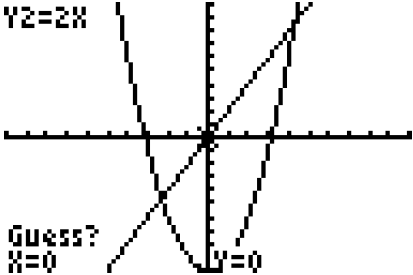
\includegraphics[scale=1.0]{Sections/SolvingEquationsGraphically/Figure13.png}
		\caption{Finding an intersection}
	\end{figure}
	
	We can see there that there are two intersections between the graphs, meaning that our equation has more than one solution. We will need to run the intersect program twice, once to get each of the shown solutions.  Now, use the arrow keys to move the blob closer to the intersection on the left. You don’t have to worry about getting really close to it, you just need to be close enough that the calculator clearly \quotes{understands} which intersection you are after. Then hitting enter to
	confirm, you get:
	
	\begin{figure}[H]
		\centering
		%should be scaled down
		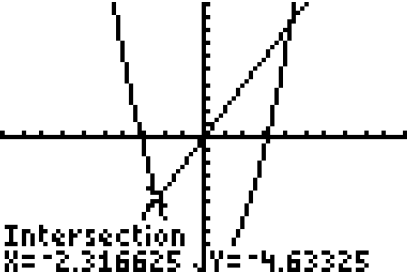
\includegraphics[scale=1.0]{Sections/SolvingEquationsGraphically/Figure14.png}
		\caption{First intersection}
	\end{figure}
	
	so one solution to the equation (rounded to two decimal places) is $x=-2.32$.\\
	
	We now need to run through the program again. Once we get to the \quotes{Guess} step, we will need to use the arrow keys to move the blob closer to the intersection on the right. We end up with:
	
	\begin{figure}[H]
		\centering
		%should be scaled down
		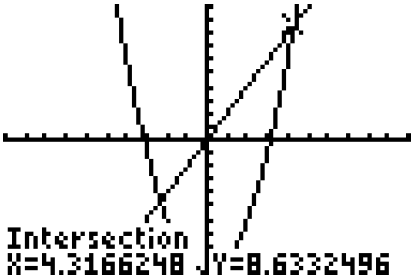
\includegraphics[scale=1.0]{Sections/SolvingEquationsGraphically/Figure15.png}
		\caption{Second intersection}
	\end{figure}
	
	So the equation’s two solutions are $x=-2.32$ and $x=4.32$.
}

%%%%%%%%%%%%%%%%%%%%%%%%%%%%%%%%%%%%%%%%%%%%%%%%%%%%%%%%%%%%
%
% Section: Solving Equations Graphically: Window Setting
%
%%%%%%%%%%%%%%%%%%%%%%%%%%%%%%%%%%%%%%%%%%%%%%%%%%%%%%%%%%%%

\subsection{Window Setting for Graphical Solution}

In all of the examples we’ve seen so far, we’ve been able to find the intersection(s) we were looking for within the standard window. Of course this won’t always happen.\\

The standard window is usually a good place to start but if the graphs you see in the standard window don’t intersect you’ll have to change the window so that you can see the intersection.  Fortunately, you’re usually not flying blind when you do this.  The graph you see in the standard window often will give you some hint about how you need to adjust.

\exam{\label{SolvingEquationsGraphicallyExample3} Solve $\frac{1}{2}x+3=\frac{x+20}{3}$ graphically}

\indenttext{We start with the standard window:
	\begin{figure}[H]
		\centering
		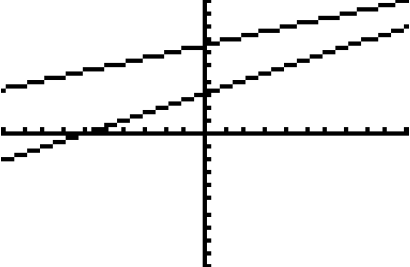
\includegraphics[scale=1.0]{Sections/SolvingEquationsGraphically/Figure16.png}
		\caption{Standard Window}
	\end{figure}

	We don’t get an intersection in the standard window, but looking at the graphs but they do appear to be coming together. If we try to run the intersect program here, though we end up with this error:
	
	\begin{figure}[H]
		\centering
		%should be scaled down
		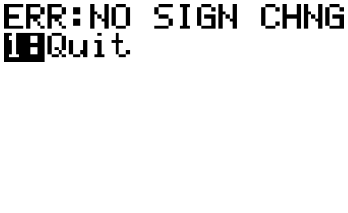
\includegraphics[scale=1.0]{Sections/SolvingEquationsGraphically/Figure17.png}
		\caption{Error screen}
	\end{figure}
	
	Not the most descriptive error code ever written, but this is the error you will get whenever you try to intersect two graphs that don’t intersect within your window’s interval of $x$-values. The intersect program will only find the intersection if it occurs within the interval of $x$-values that you have graphed. The calculator is not \quotes{smart enough} to know to look for an intersection outside that window.\\
	
	But the intersection does exist. We just have to adjust our window to find it. Looking at the graphs, we can see that they appear to be getting closer together as we move up and to the right.  So, we need to use a larger upper limit for both X and Y to find the intersection. We can’t tell how much higher we need to go, but we can make a reasonable guess and adjust as needed. Let’s try increasing both to $20$:
	
	\begin{figure}[H]
		\centering
		%should be scaled down
		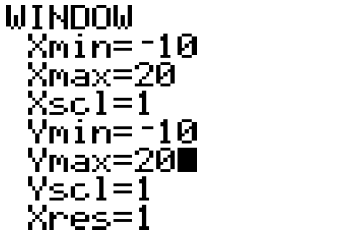
\includegraphics[scale=1.0]{Sections/SolvingEquationsGraphically/Figure18.png}
		\caption{Xmax, Ymax set from $10$ to $20$}
	\end{figure}
	
	which gives us this view of the graphs:
	
	\begin{figure}[H]
		\centering
		%should be scaled down
		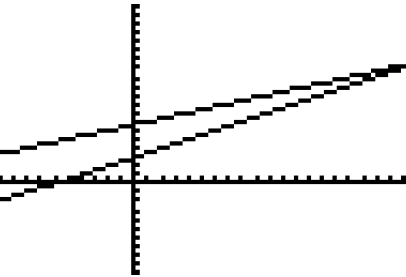
\includegraphics[scale=1.0]{Sections/SolvingEquationsGraphically/Figure19.png}
		\caption{New graph based on new window}
	\end{figure}
	
	It’s not clear whether or not they actually intersect in this window. If you try to run the Intersect program, though, you’ll see that they don’t. It doesn’t look like we need to go higher to get the intersection, but it does appear we need to go a bit farther to the right. So, adjusting Xmax up to, say, $25$, and walking through the Intersect program we end up with:
	
	\begin{figure}[H]
		\centering
		%should be scaled down
		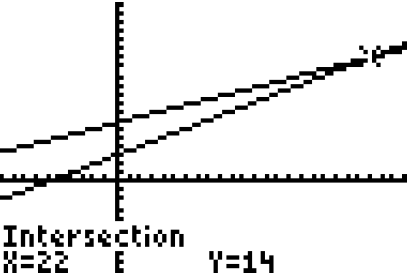
\includegraphics[scale=1.0]{Sections/SolvingEquationsGraphically/Figure20.png}
		\caption{New graph based on new window}
	\end{figure}
	
	So we can conclude the solution to this equation is $x=22$.
}

We don’t always get enough of a hint from the standard window, though. Sometimes we need to actually take a look at some values of the two functions to get a sense of a window where we might see the graphs.

\exam{\label{SolvingEquationsGraphicallyExample4} Solve $\frac{5-2x}{3}=3(2x+7)-5(x-2)$}

\indenttext{
	We start by entering the two sides of the equation as functions:

	\begin{figure}[H]
		\centering
		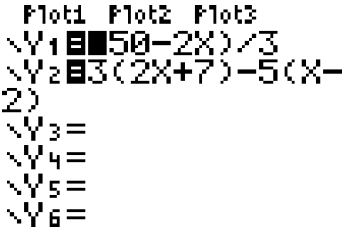
\includegraphics[scale=1.0]{Sections/SolvingEquationsGraphically/Figure21.png}
		\caption{Treating both sides as functions in the calculator}
	\end{figure}

	But if we look at these graphs in the standard window we see nothing at all! These graphs both lie entirely outside the standard window.\\
	\newline
	
	To get a hint of where to look, we can create a table. It doesn’t much matter what values we try - we’re just trying to get any glimpse of the graphs – so we’ll just use an automatic table starting at zero and going up in increments of one unit:
	
	\begin{figure}[H]
		\centering
		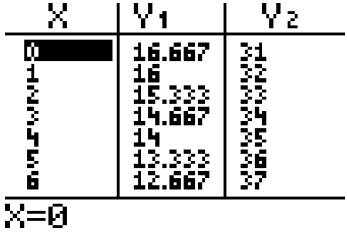
\includegraphics[scale=1.0]{Sections/SolvingEquationsGraphically/Figure22.png}
		\caption{Treating both sides as functions in the calculator}
	\end{figure}
	
	From this we can see that if we are using X-values that fall within the standard window, the Y-values are much higher than the standard window. So, we might try something like switching to \quotes{Ymin=0} and \quotes{Ymax=50}, which gives us this view:
	
	\begin{figure}[H]
		\centering
		%should be scaled down
		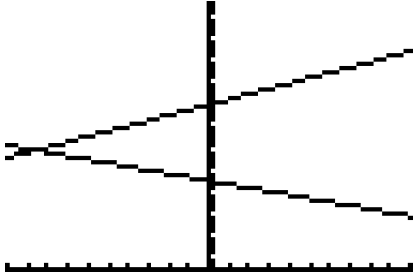
\includegraphics[scale=1.0]{Sections/SolvingEquationsGraphically/Figure23.png}
		\caption{Treating both sides as functions in the calculator}
	\end{figure}
	
	Luckily, this view not only gives us a hint where the intersection might be, it actually includes it.  Completing the process of finding the intersection, we get:
	
	\begin{figure}[H]
		\centering
		%should be scaled down
		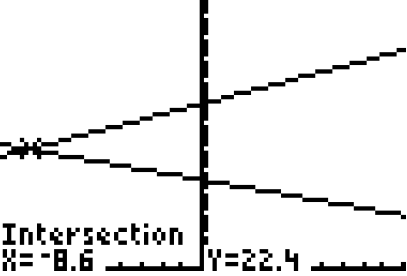
\includegraphics[scale=1.0]{Sections/SolvingEquationsGraphically/Figure24.png}
		\caption{Treating both sides as functions in the calculator}
	\end{figure}
	
	allowing us to conclude that the solution is $x=-8.6$.
}

Before concluding this discussion, there are a couple of additional points which we should address.\\

We saw in Example \ref{FunctionsandGraphsExample2} that it’s possible for an equation to have multiple solutions. Which raises the question: how do we know in Examples \ref{FunctionsandGraphsExample3} and \ref{FunctionsandGraphsExample4} that we got all the solutions? We adjusted our window to find a solution ... but how do we know that we wouldn’t find another if we looked elsewhere?\\

In both of these examples, though, we had first degree equations. We know from our prior experience of algebra that unless a first degree equation is inconsistent (no solutions) or an identity (everything is a solution) it will have one and only one solution. So, while we can’t say for sure just by looking at the graphs whether or not there are other solutions out there, what we know about algebra assures us that we don’t have to worry about this with these examples. For equations that are not first degree, such as the one in Example \ref{FunctionsandGraphsExample2}, you need to know more about how they behave algebraically and graphically to know how many solutions you are looking for. We will explore this in later chapters of this book; for the time being, if you are asked to solve an equation
that is not first degree you will be given enough additional information to know whether or not you need to look for additional solutions.\\

Another comment needs to be made about the window adjustment. It actually is not necessary to see the intersection on your calculator screen to find the intersection! The calculator requires that the solution’s input value fall inside the window in order to find the intersection, but it does not
require the output value to fall within the window. Or, said another way, the calculator cannot find the intersection if it is to the right or left of the window, but it actually can find the intersection if it falls above or below the window. So sometimes if you don’t have the intersection in the window but
run the intersect program, you get the answer anyway. This actually would have happened in Example \ref{FunctionsandGraphsExample4} if we had not adjusted the window to see the intersection. But since you can’t really rely on that happening, it’s probably best to always try to get a window that the intersection
falls within.\\

Sometimes you can get away with not seeing the intersection, sometimes you can’t. It’s safer to always try to get the intersection on screen before trying to find it.

%%%%%%%%%%%%%%%%%%%%%%%%%%%%%%%%%%%%%%%%%%%%%%%%%%%%%%%%%%%%
%
% Section: Solving Equations Graphically: When?
%
%%%%%%%%%%%%%%%%%%%%%%%%%%%%%%%%%%%%%%%%%%%%%%%%%%%%%%%%%%%%

\subsection{When to Use a Graphical Solution}

Graphical solution is a fantastically useful tool but it is not always the best approach. Often a graphical approach will allow you to solve an equation with much less effort than traditional algebra would require. And sometimes as we’ve seen it even opens up the possibility of solving equations we could not otherwise solve. But it’s also often true that graphical solution is sometimes much more work than just working through the problem with algebra.\\

For example, let’s reconsider the first equation we used as an example in this chapter:

\begin{equation*}
	2x-1=7
\end{equation*}

This can be solved either way, but I think you’ll agree that the work involved in solving this graphically was way more than the very minimal effort it takes to solve it with algebra. We used this simple equation as a first example to illustrate how graphical solution works, but in fact you almost certainly would not want to use graphical solution given the choice.\\

On the other hand, and equation like this one:

\begin{equation*}
	\frac{3}{5}x-\frac{2}{7}\left(\frac{4}{13}x+\frac{11}{3} \right) = \frac{4}{9}-\frac{2}{11}x
\end{equation*}

seems like it would take a lot of effort to work through algebraically. While it would be a pain to type each side in to the calculator, that seems like less effort than slogging through clearing all those fractions. For this equation, graphing might be a better choice.\\
\newline

Of course, there’s no hard and fast rule about this. Which method would be better to solve this one?

\begin{equation*}
	3(2x-5)-5(7+x)-9=12+4(3x-5)-2(5x+1)
\end{equation*}

On the one hand, solving this with algebra is going to involve a lot of distributing and combining like terms. Solving graphically would avoid that work. On the other hand, though, putting each side of this equation into the \quotes{Y=} screen will involve a lot of typing, and even the slightest typographical error will throw everything off. And, those are all whole numbers, which are not too bad to work with. Which approach is better? That’s really a judgment call – given the choice of methods to solve this problem, whichever one sounds preferable to you is probably the better choice for you.  Someone else might choose differently, depending on their own experience and preferences. \\
\newline

Even though there are no absolute rules here, we can make some suggestions. In general:\\
\bigskip

\begin{tabular}{|p{.5\textwidth}|p{.5\textwidth}|}
	\hline
	Traditional Algebra is Preferable if: & Graphical Solution may be Preferable if:\\
	\hline
	$\bullet$ The equation is fairly simple, requiring few steps to solve algebraically and/or & $\bullet$ The equation is complex, involving lots of distributing, combining terms, clearing fractions, or the like and/or\\
	$\bullet$ The numbers are generally whole numbers, or reasonably nice fractions or decimals and/or & $\bullet$ The numbers are \quotes{messy} decimals or fractions and/or \\
	$\bullet$ The numbers are large (making a window setting tough to find for graphical solution) and/or & $\bullet$ The numbers are not terribly large (making an appropriate window setting probably not hard to find) and/or \\
	$\bullet$ An exact answer is required and/or & $\bullet$ A rounded answer is acceptable and/or \\
	$\bullet$ The equation can be solved using algebra techniques you know & $\bullet$ The equation cannot be solved using algebra techniques you know.\\
	\hline
\end{tabular}

\exam{\label{SolvingEquationsGraphicallyExample5} Which solution method would be the better bet for each of the following equations?  Why?
	\begin{enumerate}[label=(\alph*)]
		\item $3x-5=4-2x$
		\item $4.67(2.13t-1.15)+0.87=1.13(2.22t-9.14)$
		\item $100,000x-50,000=75,000x+25,000$
		\item $\frac{3}{2}w+(4-w)=\frac{2}{5}w-3$
	\end{enumerate}
}

\indenttext{
	\begin{enumerate}[label=(\alph*)]
		\item $3x-5=4-2x$\\
		\newline

		For this, traditional algebra is probably the better bet, since solving this equation would not require too many steps and would probably be less work than  setting up and using a graph.
		\item $4.67(2.13t-1.15)+0.87=1.13(2.22t-9.14)$\\
		\newline

		The numbers in this equation are 	awkward, and solving this using traditional algebra would require quite a few steps. Graphical solution would probably be less work, though it does require being very careful to avoid typos when entering the two sides into the calculator.
		\item $100,000x-50,000=75,000x+25,000$\\
		\newline

		Here, the algebra required to solve this would 	not be terribly demanding. And since the numbers are so large it would be difficult to get an appropriate window setting for the graphs. Traditional algebra is almost certainly the better bet.
		\item $\frac{3}{2}w+(4-w)=\frac{2}{5}w-3$\\
		\newline

		This one is really a matter of preference. Because of the fractions and the simplification required, solving this one with traditional algebra will require some effort. But the fractions are not that bad and the amount of simplification required won’t be excessive so it is debatable whether that work is more or less effort than graphical solution. Either approach would be a reasonable choice.
\end{enumerate}
}

\bigskip

Sometimes you might start with one approach, and then decide that maybe it wasn’t the best approach after all. Don’t be afraid to change tactics!\\

Suppose you set out to solve this equation graphically:

\begin{equation*}
	3(2-x)+5(x-1)=3x-2(2-5x)-11x
\end{equation*}

Doing so, in the standard window you’d end up with the graph:\\

\begin{figure}[H]
	\centering
	%should be scaled down
	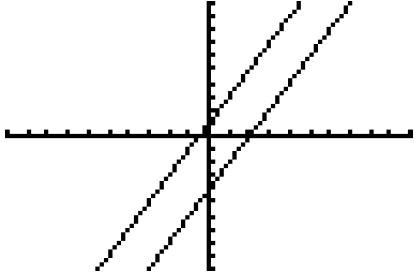
\includegraphics[scale=1.0]{Sections/SolvingEquationsGraphically/Figure25.png}
	\caption{A very hard to find intersection}
\end{figure}

Now, the two graphs don’t intersect in this window, and it’s hard to see which direction we should move if we want to find the intersection. The graphs are not coming together in any obvious way.  Now you could spend hours driving yourself crazy trying to find an appropriate window to get the intersection. Or you could just decide that maybe graphical solution won’t work so well after all. \\

Solving with algebra instead we get:

\begin{equation*}
	\begin{array}{rcl}
		3(2-x)+5(x-1)& = &3x-2(2-5x)-11x\\
		& &\\
		6-3x+5x-5&=&3x-4+10x-11x\\
		& & \\
		2x+1&=&2x-4\\
		& &\\
		1&=&-4
	\end{array}
\end{equation*}

It turns out that this is an inconsistent equation: it has no solutions. You could have spent the rest of your life looking for that intersection, and you never would have found it. Stubbornly sticking with graphical solution here would have condemned you to an eternity of futility with your graphing calculator. The horror!\\

You might object, saying that you could have seen from the initial graphs that there would never be an intersection. The graphs certainly looked like they were parallel lines, which never intersect.  Unfortunately, you can never tell that for sure just by looking at the graph. If you set out to graphically solve:

\begin{equation*}
	1.9999x+2.5=2x-1
\end{equation*}

your graphs also look like parallel lines

\begin{figure}[H]
	\centering
	%should be scaled down
	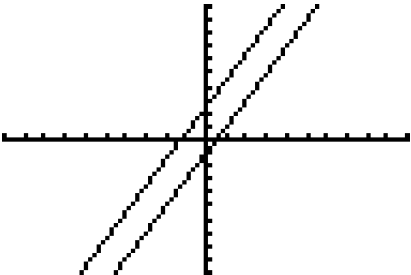
\includegraphics[scale=1.0]{Sections/SolvingEquationsGraphically/Figure26.png}
	\caption{A very hard to find intersection}
\end{figure}

But in fact this equation does have a solution:

\begin{equation*}
	\begin{array}{rcl}
		1.9999x+2.5&=&2x-1\\
		3.5&=&0.0001x\\
		x&=&35,000
	\end{array}
\end{equation*}

Just because you can’t find an intersection doesn’t mean that one doesn’t exist. These graphs actually do intersect, but you’d have to extend your window all the way out to include $x=35,000$ within the window to find it. It would take you a very long time before you’d come up with that window.\\

If you first try graphical solution and can’t find the intersection, it is incorrect to conclude that no intersection exists. It is, though, correct to conclude that maybe graphical solution isn’t the way to go.\\

In the exercises, you will find many problems where you are specifically asked to use graphical solution. If you are specifically asked to solve graphically, make sure to do so, even if you’d rather use traditional algebra. It’s important to get enough practice with this method to have it at the ready when you need it. In other exercises, though, you’ll have the choice of methods. In these, and in the future, be flexible in your approach. As we’ve seen, there are times when graphical
solution is by far the best approach, and other times where traditional algebra is the way to go. If you are comfortable with both approaches, you’ll often be able to save yourself needless exertion by having the option of choosing the easier path.

%%%%%%%%%%%%%%%%%%%%%%%%%%%%%%%%%%%%%%%%%%%%%%%%%%%%%%%%%%%%
%
% Section: Solving Equations Graphically: Exercises
%
%%%%%%%%%%%%%%%%%%%%%%%%%%%%%%%%%%%%%%%%%%%%%%%%%%%%%%%%%%%%

\clearpage

\subsection{Exercises}

\subsubsection*{Graphical Solutions}
Solve each of the following equations graphically. Some of these equations may have multiple solutions, but all solutions for these equations occur within the standard window. Round your answers to two decimal places if necessary.
\bigskip
\ex{$3+4x=5-2x$} \sol{$x=0.33$}

\bigskip
\ex{$3-2x=2x+1$}

\bigskip
\ex{$4(2-x)+3(x+1)=2(3x-1)-5x+3$} \sol{$x=5$}

\bigskip
\ex{$11x-5(2x+1)+8=4(3x+1)-2(5x-3)$}

\bigskip
\ex{$\frac{7x-11}{5}=\frac{9x+5}{2}$} \sol{$x=-1.52$}

\bigskip
\ex{$4-\frac{5}{3}x=\frac{3x+11}{5}-7$}

\bigskip
\ex{$2.31t-1.07(4.16t+3.25)=8.13+0.15(1.98t-3.17)$} 
\sol{$t=-4.57$}

\bigskip
\ex{$11.87-2.03(3.35-1.56z)=0.28(2.01z-23.95)$}

\bigskip
\ex{$2x-x^2=3x-2$} \sol{$x=1$ and $x=-2$}

\bigskip
\ex{$x^2-5x+6=5-(x-2)^2$}

\subsubsection*{Window Setting for Graphical Solution}

Solve each of the following equations graphically. You may need to adjust your window settings.  Each of these equations has one and only one solution. Round your answers to two decimal places if necessary.

\bigskip
\ex{$20-3x=9-8x$} \sol{$x=-2.2$}

\bigskip
\ex{$x+5=2x-5$}

\bigskip
\ex{$3t-28=t+4$} \sol{$t=16$}

\bigskip
\ex{$5z-35=2z+7$}

\bigskip
\ex{$\frac{19-3z}{2}=\frac{14-8z}{5}$} \sol{$z=-67$}

\bigskip
\ex{$\frac{4t-3}{5}=\frac{3t+7}{4}$}

\bigskip
\ex{$2y+10=\frac{3}{2}y-10$} \sol{$y=-40$}

\bigskip
\ex{$\frac{5}{3}y+8=\frac{6}{5}y-12$}

\bigskip
\ex{$2x+1=20-x$} \sol{$x=6.33$}

\bigskip
\ex{$3x-5=30-2x$}

\bigskip
\ex{$\frac{3x+50}{2}=\frac{2x+70}{5}$} \sol{$x=-10$}

\bigskip
\ex{$\frac{3-2x}{5}-11=\frac{40-x}{2}$}

\subsubsection*{When to use graphical solutions}

For each of the following questions, decide whether you would rather try to solve using graphical solution or traditional algebra. Do not actually solve the equations. The better method is a matter of opinion, so there are no right or wrong answers, but you should explain your reasoning.

\bigskip
\ex{$3.25(4.13x-3.17)-2.55=0.87x+3.13(0.55x-1.15)$} \sol{Graphically since the algebra looks lengthy.}

\bigskip
\ex{$\frac{3}{5}(\frac{2}{3}t-\frac{7}{5})-\frac{11}{12}=\frac{5}{4}-\frac{8}{11}(3-\frac{2}{5}t)$}

\bigskip
\ex{$4x-2=3x+1$} \sol{Algebraically, it looks quick to solve.}

\bigskip
\ex{$1250z+25,000=300(40z-12,000)$}

\bigskip
\ex{$5(3-y)=2(6+y)-5(2y+7)$} \sol{Either, algebraically is reasonable and graphical would not take too long.}

\bigskip
\ex{$3x+2=17$}

\bigskip
\ex{$\frac{r-2}{3}=\frac{r+9}{5}$} \sol{Algebraically, as long as fractions are not terrible it is preferable}

\bigskip
\ex{$z^2-5z+3=2z+1$}

\bigskip
\ex{$3z^2-5z+3=8-z^2$} \sol{Graphically, it is easier to find both solutions visually}

\bigskip
\ex{$\frac{1}{3}t-\frac{4}{5}=7-\frac{9}{2}t$}

\subsubsection*{Grab Bag}

Solve each of these equations either graphically or using traditional algebra. Choose the most efficient solution method – do not work harder than you need to! Unless otherwise noted, each of these equations has only one solution. Round your answers to two decimal places if necessary.

\bigskip
\ex{$2(3x-1)-5x=8x+3-3(2x+5)$} \sol{$x=10$}

\bigskip
\ex{$1.43x-3.79=2.05(1.17x-5.13)$}

\bigskip
\ex{$500t-23,000=15(30t-200)$} \sol{$t=400$}

\bigskip
\ex{$\frac{3x-7}{5}=\frac{2x+1}{3}+1$}

\bigskip
\ex{$8.62x-3.09(1.89x-2.19)=9.87-2.01(0.76x+1.52)$} \sol{$x=0.01$}

\bigskip
\ex{$2w-1=9$}

\bigskip
\ex{$18-2t-(t-8)=3(t-9)-2(t-5)$} \sol{$t=10.75$}

\bigskip
\ex{$\frac{7}{3}x-\frac{29}{2}=\frac{3}{2}x-\frac{62}{3}$}

\bigskip
\ex{$x^2-2x+8=8$} \quad (NOTE: This equation has two solutions.) \sol{$x=0$ and $x=2$}

\bigskip
\ex{$180k-32,000=160k+48,000$}

\bigskip
\ex{$3(2t-5)-3(t-2)=5t+7-2(t+1)$} \sol{No Solutions}

\bigskip
\ex{$z^2=3z+1$} \quad (NOTE: This equation has two solutions.)

\bigskip
\ex{$\frac{19x-5}{10}=\frac{39x+50}{40}$} \sol{$x=1.89$}

\bigskip
\ex{$5(2-x)+7=3(4-x)+1$}

\bigskip
\ex{$8x-3(2x+5)=x+1$} \sol{$x=16$}

\bigskip
\ex{$40-3x=5(x+3)-3(x-12)$}

\bigskip
\ex{$1.03y+2.01(1.13y-1.45)=11.02-2.86(1.72y-0.14)$} \sol{$x=1.74$}

\bigskip
\ex{Suppose $S$ is a rule that takes equations as inputs and gives their solutions as outputs. Is $S$ is function? Why or why not?}

\clearpage
